\documentclass[10pt,aspectratio=1610,compress,dvipsnames]{beamer}

\makeatletter
\def\input@path{{tex/}{chapters/}}
\makeatother

\usetheme[]{CodingTealArc}

%-------------------------------------------------------
% PACKAGES
%-------------------------------------------------------

\usepackage{helvet}
\usepackage{fontspec}
\usepackage{unicode-math}
\setmainfont{TeX Gyre Termes}
\setmathfont{TeX Gyre Pagella Math}

\setsansfont[
Path = fonts/,
UprightFont = *Medium.ttf,
BoldFont    = *Bold.ttf
]{GmarketSansTTF}
\usepackage{textcomp}
\renewcommand{\ttdefault}{lmtt}

\newcommand{\chref}[2]{
  \href{#1}{{\usebeamercolor[bg]{CodingTealArc} #2}}
}

\makeatletter
\def\blfootnote{\gdef\@thefnmark{}\@footnotetext}
\makeatother

\usepackage{listings}
\usepackage{tikz}
\usepackage{pgfplots, pgfplotstable}
\pgfplotsset{compat=1.18}
\usetikzlibrary{
  3d,
  angles,
  arrows,
  arrows.meta,
  backgrounds,
  bending,
  calc,
  decorations.pathmorphing,
  decorations.pathreplacing,
  decorations.markings,
  fit,
  matrix,
  patterns,
  patterns.meta,
  positioning,
  shadows,
  shapes,
  shapes.geometric,
  tikzmark,
  quotes
}
\usetikzlibrary{mindmap}

\usepackage{multicol}
\renewcommand{\lstlistingname}{Code}
\usepackage{array}
\usepackage{booktabs}
\usepackage{adjustbox}
\usepackage{kotex}
\usepackage{soul}
\usepackage{colortbl}

%-------------------------------------------------------
% TITLE PAGE INFORMATION
%-------------------------------------------------------

\definecolor{myteal}{HTML}{008C8C}
\definecolor{mydarkteal}{HTML}{003F46}

\title[Code-Based Hard Problems]
{
  \texorpdfstring{\textbf{\Huge\color{myteal!70!black} Code-Based Hard Problems}}{Code-Based Hard Problems}
}
\subtitle[Syndrome Decoding and Quasi-Cyclic Variants]
{
  \texorpdfstring{\text{\LARGE -- Syndrome Decoding \& Quasi-Cyclic Variants --}}{Syndrome Decoding and Quasi-Cyclic Variants}
}

\author[Ji, Yong-hyeon]
{\texorpdfstring{
  \vspace{.5cm}
  {\centering
    
\includegraphics[scale=1.5]{tikzs/jyh.pdf}
  }\\ [-.2cm]
}{Ji, Yong-hyeon}}

\institute[Enjoying Math]
{
  \vspace{-.5cm}
  \textbf{\Large PQC Hard Problem Colloquium}\\
  \vspace{-0.5cm}
  \vspace{1cm}
  \textbf{\large\it 2026 Spring}\\
  \vspace{-1cm}
}

\date{\today}

\usepackage{tcolorbox}
\tcbset{colback=white, arc=5pt}

% teal-family colors for math boxes
\definecolor{axiomcolor}{HTML}{00646A}
\definecolor{defcolor}{HTML}{007575}
\definecolor{procolor}{HTML}{00575E}
\definecolor{thmcolor}{HTML}{003F46}
\definecolor{lemcolor}{HTML}{006F73}
\definecolor{corcolor}{HTML}{00615F}
\definecolor{execolor}{HTML}{004F54}

\newcommand{\axiombox}[2][]{%
  \begin{tcolorbox}[colframe=axiomcolor, title={\color{white}\bfseries #1}]
    #2
  \end{tcolorbox}
}
\newcommand{\defbox}[2][]{%
  \begin{tcolorbox}[colframe=defcolor, title={\color{white}\bfseries #1}]
    #2
  \end{tcolorbox}
}
\newcommand{\lembox}[2][]{%
  \begin{tcolorbox}[colframe=lemcolor, title={\color{white}\bfseries #1}]
    #2
  \end{tcolorbox}
}
\newcommand{\probox}[2][]{%
  \begin{tcolorbox}[colframe=procolor, title={\color{white}\bfseries #1}]
    #2
  \end{tcolorbox}
}
\newcommand{\thmbox}[2][]{%
  \begin{tcolorbox}[colframe=thmcolor, title={\color{white}\bfseries #1}]
    #2
  \end{tcolorbox}
}
\newcommand{\corbox}[2][]{%
  \begin{tcolorbox}[colframe=corcolor, title={\color{white}\bfseries #1}]
    #2
  \end{tcolorbox}
}
\newcommand{\exebox}[2][]{%
  \begin{tcolorbox}[colframe=execolor, title={\color{white}\bfseries #1}]
    #2
  \end{tcolorbox}
}

\usepackage{listings}
%\definecolor{type}{HTML}{4EC9B0} %  A turquoise or teal.
\definecolor{atompurple}{rgb}{0.7, 0.4, 0.8}
\definecolor{keyword}{HTML}{8e4e9e}
\definecolor{myblue}{HTML}{3471d8}
\definecolor{type}{HTML}{4EC9B0}
\definecolor{golden}{HTML}{d19a66}

% Change "Listing" to another name, e.g., "Code"
\renewcommand{\lstlistingname}{Code}
\lstdefinestyle{normal}{
	frame=single, % Border
	basicstyle=\tt\small, % Code font style
	breaklines=true, % Break long lines into multiple lines automatically
	aboveskip=1.5\baselineskip, % Vertical whitespace before the listing
	tabsize=3, % How many space to a tab
}
\lstdefinestyle{shell}{
	keywordstyle={\bfseries\color{JungleGreen}},
	morekeywords={jasminc, -ec},
	%	numbers=left, % Line numbers location
	%	numbersep=6pt, % Whitespace to the right of line numbers
	%	numberstyle=\tiny\it, % Line numbers font style
	linewidth=\textwidth,  % Sets the listing width to match the text width
	frame=single, % Border
	basicstyle=\tt\scriptsize, % Code font style
	breaklines=true, % Break long lines into multiple lines automatically
	aboveskip=1.5\baselineskip, % Vertical whitespace before the listing
	tabsize=2, % How many space to a tab
}
\lstdefinestyle{c}{
	language=C,
	basicstyle=\ttfamily\small,        % Basic font style
	keywordstyle=\color{keyword}\bfseries,       % Keywords in bold blue
	keywordstyle=[2]\color{myblue}\bfseries,
	keywordstyle=[3]\color{magenta}\bfseries,
	keywordstyle=[4]\color{purple}\bfseries,
	stringstyle=\color{red!70},               % Strings in reddish color
	commentstyle=\color{green!50!black}\itshape, % Comments in italic green-black
	numberstyle=\tiny\color{gray},            % Line numbers in tiny gray font
	numbers=left,                             % Line numbers on the left
	stepnumber=1,                             % Number every line
	numbersep=8pt,                            % Space between line numbers and code
%	backgroundcolor=\color{gray!10},          % Light gray background
	frame=single,                             % Single-line frame around the code
	rulecolor=\color{gray},                   % Frame color
	tabsize=4,                                % Tab space width
	showstringspaces=false,                   % Don't show spaces in strings
	breaklines=true,                          % Line breaking enabled
	breakatwhitespace=true,                   % Break lines at whitespace
	captionpos=b,                             % Caption below the code
	escapeinside={\%*}{*)},                   % Allow LaTeX within code
	morekeywords={printf, scanf, main, size_t, uint8_t, uint16_t, uint32_t, uint64_t},
	morekeywords=[2]{randomSeed, hashArray,
	expandChallenge, expandATF_vec_copy, expandColumns, expandSeeds,
	invertingOnATF, actingOnATFS, columnsMatrix, columnsDecomposition,
	multiplicationModuloP, addmul_P32_into_64, reductionModuloP,
	reductionStrict, inversionModuloP},
	morekeywords=[3]{crypto_sign_keypair, crypto_sign},
	morekeywords=[4]{lu}
}
% Command to Include Rust Code
\newcommand{\ccode}[2][]{%
	\lstinputlisting[style=c,#1]{#2}
}

% Inline Code Highlighting
\newcommand{\cinline}[1]{%
	\lstinline[style=c]|#1|%
}
\lstdefinestyle{asm}{
	%	language=[x86masm]Assembler,
	language=C,
	basicstyle=\ttfamily\small,
	keywordstyle=\color{blue},
	commentstyle=\color{gray!50},
	stringstyle=\color{orange},
	morekeywords={.data, .align, .asciz, .text, .global, .type, .size, .extern, stp, mov, adr, ldr, add, bl, ret, ldp, and,
	movk, lsr, mul, sub, uxtw, cmp, blt, str, cbnz},
	numbers=none,
	frame=single,                             % Single-line frame around the code
	rulecolor=\color{gray},                   % Frame color
}

%\lstdefinestyle{jasmin}{
%	language=[x86masm]Assembler, % Closest to Jasmin syntax
%	basicstyle=\ttfamily\small, % Monospace font for code
%	keywordstyle=\color{blue}\bfseries, % Keywords in blue and bold
%	stringstyle=\color{orange}, % Strings in orange
%	commentstyle=\color{green!60!black}\itshape, % Comments in green
%	numbers=left, % Line numbers on the left
%	numberstyle=\tiny\color{gray}, % Line number style
%	stepnumber=1, % Show every line number
%	numbersep=5pt, % Space between numbers and code
%	frame=single, % Single frame around code
%	tabsize=4, % Tab width
%	showstringspaces=false, % Don't underline spaces in strings
%	breaklines=true, % Wrap long lines
%	captionpos=b, % Caption at the bottom
%	morekeywords={mov, add, sub, mul, xor, and, or, shl, shr, call, ret, lea}, % Add Jasmin-specific keywords
%	escapeinside={(*@}{@*)} % For embedding LaTeX inside code
%}



%
%% --------------------------------------------------------------------
%\newcommand{\dslash}{\mathbin{\mathsf{/\mkern-4mu/}}}
%\newcommand{\dslasheq}{\mathbin{\mathsf{/\mkern-4mu/\mkern-8mu=}}}
%\newcommand{\slasheq}{\mathbin{\mathsf{/\mkern-6mu=}}}

% --------------------------------------------------------------------
\definecolor{OliveGreen}{rgb}{0.33, 0.5, 0.18}
\definecolor{Blue}{rgb}{0.06, 0.2, 0.65}
\definecolor{grey}{rgb}{0.43, 0.5, 0.5}
\lstdefinestyle{jasmin}{
	mathescape=true,
	columns=fullflexible,
	keepspaces=true,
	captionpos=b,
	frame=tb,
%	xleftmargin=.1\textwidth,
%	xrightmargin=.1\textwidth,
	rangebeginprefix={(**\ begin\ },
	rangeendprefix={(**\ end\ },
	rangesuffix={\ *)},
	includerangemarker=false,
	basicstyle=\small\sffamily,
	identifierstyle={},
	keywordstyle=[1]{\color{OliveGreen}},
	keywordstyle=[2]{\color{keyword}\bfseries},
	keywordstyle=[3]{\color{Blue}},
	keywordstyle=[4]{\bfseries\color{OliveGreen}},
	keywordstyle=[5]{\color{Red}},
	keywordstyle=[6]{\color{golden}},
	keywordstyle=[7]{\bfseries\color{magenta}},
%	morekeywords=[7]{xor, aes, enc, dec},
	morekeywords=[2]{fn,for,to,downto,if,else,do,while,return,param},
	morekeywords=[3]{u256,u128,u64,u32,u16,u8,bool,int},
	morekeywords=[1]{reg,stack,inline,export},
	comment=[l][\color{grey}]{//},
	morecomment=[s][\color{grey}]{/*}{*/},
	alsoletter ={_},
	literate=
	{-}{-}{1}%
	{->}{$\rightarrow$}{1}%
	{4u64}{4u64}{1}%
	{>>}{$\gg$}{1}%
	{<<}{$\ll$}{1}%,
}[keywords,comments]
\newcommand{\jasmincode}[2][]{%
	\lstinputlisting[style=jasmin,#1]{#2}
}
\newcommand{\jasmininline}[1]{%
	\lstinline[style=jasmin]|#1|%
}

\newcommand{\dslash}{\mathbin{\mathsf{/\mkern-4mu/}}}
\newcommand{\dslasheq}{\mathbin{\mathsf{/\mkern-4mu/\mkern-8mu=}}}
\newcommand{\slasheq}{\mathbin{\mathsf{/\mkern-6mu=}}}
\newcommand{\drarrow}{\raisebox{.07em}{$\mathbin{\scriptstyle\mathsf{-\mkern-3mu>}}$}}
\newcommand{\dlarrow}{\raisebox{.07em}{$\mathbin{\scriptstyle\mathsf{<\mkern-3mu-}}$}}
\newcommand{\drrarrow}{\raisebox{.07em}{$\mathbin{\scriptstyle\mathsf{-\mkern-3mu>\mkern-3mu>}}$}}
\newcommand{\dllarrow}{\raisebox{.07em}{$\mathbin{\scriptstyle\mathsf{<\mkern-3mu<\mkern-3mu-}}$}}
\lstdefinestyle{easycrypt}{
	upquote=true,
	escapechar=\#,
	mathescape=false,
	columns=fullflexible,
	keepspaces=true,
	captionpos=b,
	frame=tb,
%	xleftmargin=.1\textwidth,
%	xrightmargin=.1\textwidth,
	rangebeginprefix={(**\ begin\ },
	rangeendprefix={(**\ end\ },
	rangesuffix={\ *)},
	includerangemarker=false,
	basicstyle=\small\ttfamily,
	identifierstyle={},
	keywordstyle=[1]{\bfseries\color{violet}},
	keywordstyle=[2]{\bfseries\color{olive}},
	keywordstyle=[3]{\bfseries\color{blue}},
	keywordstyle=[4]{\bfseries\color{blue}},
	keywordstyle=[5]{\bfseries\color{red}},
	keywordstyle=[6]{\bfseries\color{violet}},
	morekeywords=[1]{arg},
	morecomment=[n][\itshape]{(*}{*)},
	morecomment=[n][\bfseries]{(**}{*)},
	morekeywords=[1]{forall,exists,fun,glob,let,in,var,proc,if,then,else,elif,while,assert,return,res,equiv,hoare,phoare,islossless,async},
	morekeywords=[2]{axiom,axiomatized,lemma,realize,proof,qed,abort,goal,end,import,export,include,local,declare,hint,nosmt,module,of,const,op,pred,inductive,notation,abbrev,require,theory,abstract,section,type,class,instance,print,search,as,Pr,clone,with,rename,prover,timeout,why3,dump,remove,Top,Self},
	morekeywords=[3]{beta,iota,zeta,eta,logic,delta,simplify,congr,change,split,left,right,case,pose,cut,have,suff,elim,clear,wlog,apply,rewrite,rwnormal,subst,progress,trivial,auto,idtac,move,modpath,field,fieldeq,ring,ringeq,algebra,replace,transitivity,symmetry,seq,wp,sp,sim,skip,call,rcondt,rcondf,swap,cfold,rnd,pr_bounded,bypr,byphoare,byequiv,fel,conseq,exfalso,inline,alias,fission,fusion,unroll,splitwhile,kill,eager},
	morekeywords=[4]{try,first,last,do,strict,expect},
	morekeywords=[5]{exact,assumption,smt,by,reflexivity,done,solve},
	morekeywords=[6]{admit,admitted},
	literate=
	{tau}{$\tau$}1
	{sigma}{$\sigma$}1
	% note double "_" below
	% in actual EasyCrypt examples, do not use __
	% in specifications, these are rendered as subscripts
	{__1}{${}_{\!1}$}1
	{__2}{${}_{\!2}$}1
	{__3}{${}_{\!3}$}1
	{__n}{${}_{\!n}$}1
	{__p}{${}_{\!p}$}1
	{,,,}{$\mathrel{\ldots}$}1
	{...}{$\mathrel{\cdots}$}1
	{->}{$\drarrow$}1
	{<-}{$\dlarrow$}1
	{->>}{$\drrarrow$}2
	{<<-}{$\dllarrow$}2
}
\newcommand{\easycryptcode}[2][]{%
	\lstinputlisting[style=easycrypt,#1]{#2}
}
\newcommand{\easycryptinline}[1]{%
	\lstinline[style=easycrypt]|#1|%
}


%\lstdefinestyle{easycrypt}{
%	language=ML, % EasyCrypt syntax is close to ML
%	basicstyle=\ttfamily\small, % Monospace font for code
%	keywordstyle=\color{purple}\bfseries, % Keywords in purple and bold
%	commentstyle=\color{green!60!black}, % Comments in green
%	stringstyle=\color{orange}, % Strings in orange
%	numbers=left, % Line numbers on the left
%	numberstyle=\tiny\color{gray}, % Line number style
%	stepnumber=1, % Show every line number
%	numbersep=5pt, % Space between numbers and code
%	frame=single, % Single frame around code
%	tabsize=4, % Tab width
%	showstringspaces=false, % Don't underline spaces in strings
%	breaklines=true, % Wrap long lines
%	captionpos=b, % Caption at the bottom
%	morekeywords={module, axiom, lemma, theorem, proof, qed, fun, let, in, forall, exists, if, then, else, return, assume, while, do, match, with}, % EasyCrypt-specific keywords
%	escapeinside={(*@}{@*)} % For embedding LaTeX inside code
%}
%\newcommand{\easycryptcode}[2][]{%
%	\lstinputlisting[style=easycrypt,#1]{#2}
%}
%\newcommand{\easycryptinline}[1]{%
%	\lstinline[style=easycrypt]|#1|%
%}
% Pseudo-code
\usepackage[linesnumbered,ruled]{algorithm2e}
\usepackage{algorithmicx}
\usepackage{algpseudocode}
%\usepackage{setspace}
\SetKwComment{Comment}{/* }{ */}
\SetKwProg{Fn}{Function}{:}{end}
\SetKwProg{Procedure}{Procedure}{:}{end}
\SetKw{End}{end}
\SetKw{DownTo}{downto}
% -- math shorthands ----------------------------------------------------------

\newcommand{\F}{\mathbb{F}}
\newcommand{\Z}{\mathbb{Z}}
\newcommand{\N}{\mathbb{N}}
\newcommand{\Q}{\mathbb{Q}}
\newcommand{\R}{\mathbb{R}}
\newcommand{\C}{\mathbb{C}}

\newcommand{\set}[1]{\left\{#1\right\}}
\newcommand{\abs}[1]{\left|#1\right|}
\newcommand{\norm}[1]{\left\lVert #1\right\rVert}
\newcommand{\inner}[2]{\left\langle #1,#2\right\rangle}
\newcommand{\gen}[1]{\left\langle #1\right\rangle}
\newcommand{\ideal}[1]{\left\langle #1\right\rangle}
\newcommand{\vect}[1]{\mathbf{#1}}
\newcommand{\mat}[1]{\mathbf{#1}}

% -- coding theory shorthands -------------------------------------------------

\newcommand{\code}{\mathcal{C}}
\newcommand{\wt}{\operatorname{wt}}
\newcommand{\rank}{\operatorname{rank}}
\newcommand{\Span}{\operatorname{span}}
\newcommand{\supp}{\operatorname{supp}}
\newcommand{\poly}{\operatorname{poly}}
\newcommand{\negl}{\operatorname{negl}}
\newcommand{\ol}[1]{\overline{#1}}

\newcommand{\nkcode}[3]{[#1,#2]_{#3}}
\newcommand{\nkdcode}[4]{[#1,#2,#3]_{#4}}

% -- presentation teaching lens -----------------------------------------------

\newcommand{\hardproblemlens}{%
  Code-based hardness lives in the gap between linear algebra and combinatorial search.%
}
\newcommand{\HardProblemLens}[1]{%
  \gdef\hardproblemlens{#1}%
}

% -- colors -------------------------------------------------------------------

\definecolor{accent}{HTML}{1F4E79}
\definecolor{softaccent}{HTML}{EAF2F8}
\definecolor{softgray}{HTML}{F6F7F9}
\definecolor{successdraw}{HTML}{27AE60}
\definecolor{successfill}{HTML}{EAFAF1}
\definecolor{errordraw}{HTML}{C0392B}
\definecolor{errorfill}{HTML}{FDEDEC}

\definecolor{Ink}{HTML}{101A24}
\definecolor{Paper}{HTML}{F8FBFC}
\definecolor{Grid}{HTML}{DCEAEC}
\definecolor{BlueCode}{HTML}{3155A4}
\definecolor{AmberCode}{HTML}{B87511}
\definecolor{ErrorRed}{HTML}{D33F49}
\definecolor{GoodGreen}{HTML}{3C8D4F}
\definecolor{VioletCode}{HTML}{6E5AA8}

% -- tikz styles --------------------------------------------------------------

\tikzset{
  every picture/.style={
    font=\sffamily,
    line cap=round,
    line join=round
  },
  title text/.style={
    font=\sffamily\bfseries\large,
    text=TealDarkCyan
  },
  caption text/.style={
    font=\sffamily\small,
    text=Ink!72
  },
  tiny label/.style={
    font=\sffamily\scriptsize,
    text=Ink!72
  },
  bit/.style={
    draw=TealDarkCyan!55,
    fill=Paper,
    minimum width=0.46cm,
    minimum height=0.46cm,
    inner sep=0pt,
    font=\sffamily\scriptsize\bfseries
  },
  bit teal/.style={
    bit,
    fill=AccentCyan!13,
    draw=AccentCyan!75,
    text=TealDarkCyan
  },
  bit blue/.style={
    bit,
    fill=BlueCode!12,
    draw=BlueCode!72,
    text=BlueCode!85!black
  },
  bit amber/.style={
    bit,
    fill=AmberCode!15,
    draw=AmberCode!72,
    text=AmberCode!85!black
  },
  bit error/.style={
    bit,
    fill=ErrorRed!13,
    draw=ErrorRed!80,
    text=ErrorRed!85!black
  },
  panel/.style={
    draw=TealDarkCyan!26,
    fill=Paper,
    rounded corners=3pt,
    line width=0.8pt,
    inner sep=6pt
  },
  process/.style={
    draw=TealDarkCyan!68,
    fill=TealDarkCyan!7,
    rounded corners=3pt,
    line width=0.9pt,
    align=center,
    inner sep=6pt
  },
  process blue/.style={
    process,
    draw=BlueCode!70,
    fill=BlueCode!8,
    text=BlueCode!80!black
  },
  process amber/.style={
    process,
    draw=AmberCode!75,
    fill=AmberCode!10,
    text=AmberCode!80!black
  },
  process red/.style={
    process,
    draw=ErrorRed!75,
    fill=ErrorRed!9,
    text=ErrorRed!85!black
  },
  flow/.style={
    -{Stealth[length=3.0pt]},
    line width=0.95pt,
    draw=TealDarkCyan!80
  },
  flow blue/.style={
    flow,
    draw=BlueCode!80
  },
  flow amber/.style={
    flow,
    draw=AmberCode!82
  },
  flow red/.style={
    flow,
    draw=ErrorRed!80
  }
}


\begin{document}

%-------------------------------------------------------
% TITLE PAGE
%-------------------------------------------------------
\HardProblemLens{The syndrome of a linear code is the pivot: it enables perfect decoding, and it hides the hard problem.}
\begin{frame}[plain,noframenumbering]
  \titlepage
\end{frame}

%-------------------------------------------------------
% TABLE OF CONTENTS
%-------------------------------------------------------
\section*{Contents}
\HardProblemLens{The story moves from easy algebraic decoding to hard random decoding, then to the compact quasi-cyclic compromise.}
\begin{frame}{\textbf{Contents}}
  \tableofcontents
\end{frame}

%-------------------------------------------------------
% I. INTRODUCTION
%-------------------------------------------------------
\section{I. Introduction}
\HardProblemLens{The same linear algebra that makes decoding easy for Hamming codes makes it hard for random codes.}
%=======================================================
% CHAPTER 0: INTRODUCTION
%=======================================================

\begin{frame}[plain]
  \begin{center}\bfseries\centering
    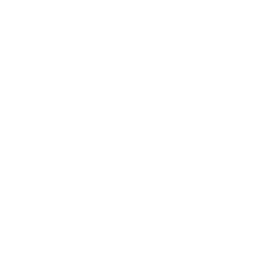
\includegraphics[scale=1]{assets/branding/opa0}
    \vspace{-5.75cm}\\
    {\adjustbox{scale=2.5}{\color{TealDarkCyan}\;I.\;Introduction}}
    \vspace{.25cm}
    \begin{minipage}{.78\textwidth}
      \scriptsize\color{Ink}
      \textbf{Big picture.}\;
      The syndrome of a linear code is a simple linear map — and it is both the key to perfect decoding and the source of a hard cryptographic problem.\\[.2cm]
      \textbf{Details to watch.}\;
      parity-check matrix, syndrome, algebraic structure, NP-hardness, quasi-cyclic.
    \end{minipage}
    {\ }\vspace{2.1cm}\\
    \bigskip
  \end{center}
\end{frame}

%--- Two faces of one object ---
\begin{frame}{\textbf{I. Introduction}}{The Same Object, Two Different Questions}
\small
\begin{columns}[T,onlytextwidth]
\begin{column}{.48\textwidth}
\textcolor{TealDarkCyan}{\textbf{Face 1: Reliable Communication}}
\begin{itemize}
  \item A linear code $\code\le\F_q^n$ adds \emph{known} redundancy.
  \item Channel adds an \emph{unknown} error $\vect e$.
  \item Syndrome $\vect s = \mat H\vect e^T$ reveals $\vect e$.
  \item \textbf{Goal}: recover $\vect e$ quickly — and then correct it.
\end{itemize}
\end{column}
\begin{column}{.48\textwidth}
\textcolor{TealDarkCyan}{\textbf{Face 2: Public-Key Cryptography}}
\begin{itemize}
  \item A random $\mat H$ hides a \emph{secret} sparse $\vect e$.
  \item Adversary sees only $\mat H$ and $\vect s = \mat H\vect e^T$.
  \item No algebraic shortcut exists for a random $\mat H$.
  \item \textbf{Goal}: make recovery computationally infeasible.
\end{itemize}
\end{column}
\end{columns}
\bigskip
\begin{center}
\begin{tikzpicture}[node distance=.72cm]
  \node[process,minimum width=2.8cm] (H) {$\mat H\in\F_q^{r\times n}$\\[-1pt]\scriptsize parity-check matrix};
  \node[process blue,  right=1.4cm of H]  (synd)  {syndrome\\$\vect s=\mat H\vect e^T$};
  \node[process amber, above right=.4cm and 1.4cm of synd] (easy)
    {structured $\mat H$\\$\Rightarrow$ fast decoder};
  \node[process red,   below right=.4cm and 1.4cm of synd] (hard)
    {random $\mat H$\\$\Rightarrow$ NP-hard};
  \draw[flow]       (H)     -- (synd);
  \draw[flow amber] (synd.north east) -- (easy);
  \draw[flow red]   (synd.south east) -- (hard);
\end{tikzpicture}
\end{center}
\end{frame}

%--- The decoding gap ---
\begin{frame}{\textbf{I. Introduction}}{The Decoding Gap}
\scriptsize
\begin{columns}[T,onlytextwidth]
\begin{column}{.56\textwidth}
\defbox[Q. Why does structure matter so much?]{
\textbf{Hamming code.}\;
For $\mat H_3\in\F_2^{3\times 7}$ — columns are all nonzero binary vectors of length 3 —
the syndrome $\vect s = \mat H_3\vect e^T$ \emph{is} the binary address of the error position.
Decoding is a single look-up: $O(1)$ time.

\medskip
\textbf{Random code.}\;
For a random $\mat H\in\F_2^{r\times n}$, the same equation $\mat H\vect e^T = \vect s$ with $\wt(\vect e)=w$
defines the \textbf{Syndrome Decoding Problem}.
The best algorithms run in time $\approx 2^{0.054n}$ — exponential for large $n$.

\medskip
\textbf{What changes?}\;
Nothing in the equation.
Everything in the matrix structure.}
\end{column}
\begin{column}{.40\textwidth}
\begin{center}
\begin{tikzpicture}[scale=.64]
  % Axis: structure on x, decoding cost on y
  \draw[->,Ink!60] (-.2,0) -- (4.5,0)
    node[right,tiny label]{structure};
  \draw[->,Ink!60] (0,-.2) -- (0,3.6)
    node[above,tiny label]{decoding cost};
  % Curve: high cost at left (random), near zero at right (structured)
  \draw[TealDarkCyan,thick,domain=0.2:4.0,samples=40]
    plot (\x, {3.2*exp(-0.9*\x)});
  % Annotations
  \fill[ErrorRed] (0.35,2.55) circle (2.8pt);
  \node[right,tiny label,ErrorRed!80] at (0.5,2.7) {random: $2^{0.054n}$};
  \fill[GoodGreen] (3.5,0.15) circle (2.8pt);
  \node[right,tiny label,GoodGreen] at (3.6,0.3) {Hamming: $O(1)$};
  \fill[BlueCode] (2.1,0.65) circle (2.8pt);
  \node[right,tiny label,BlueCode] at (2.2,0.85) {QC: $2^{0.054m}$};
  \node[caption text,align=center] at (2.2,-0.65)
    {more algebraic structure $\to$ faster decode};
\end{tikzpicture}
\end{center}
\end{column}
\end{columns}
\end{frame}

%--- The central characters ---
\begin{frame}{\textbf{I. Introduction}}{The Central Characters}
\small
\begin{center}
\renewcommand{\arraystretch}{1.28}
\begin{tabular}{>{\bfseries}p{.22\textwidth}p{.35\textwidth}p{.30\textwidth}}
\toprule
Code family & Structure & Decoding \\
\midrule
Hamming $[2^r-1,2^r-1-r,3]_2$ & Projective parity checks & Syndrome = error address; $O(1)$ \\
Cyclic (BCH, RS) & Polynomial ideal in $R_n$ & Root syndromes; polynomial-time \\
QC-MDPC (BIKE) & Circulant blocks in $R_m^\ell$ & Iterative bit-flipping; probabilistic \\
Random linear code & None & SDP; best known $2^{0.054n}$ \\
\bottomrule
\end{tabular}
\end{center}
\bigskip
\textbf{The pattern.}
More algebraic structure enables a more direct decoder —
and makes the code unsuitable as a cryptographic primitive.
Random codes have no efficient decoder and are the right hardness engine.
\end{frame}

%--- Roadmap ---
\begin{frame}{\textbf{I. Introduction}}{Roadmap: A Four-Act Story}
\small
\begin{center}
\begin{tikzpicture}[node distance=.6cm]
  \node[process,minimum width=3.2cm,align=center]
    (act1) {\textbf{Act I (here)}\\Introduction\\Two faces of a syndrome};
  \node[process blue,right=.85cm of act1,minimum width=3.2cm,align=center]
    (act2) {\textbf{Act II}\\When Decoding\\Is \emph{Easy}\\(Hamming, Cyclic)};
  \node[process amber,right=.85cm of act2,minimum width=3.2cm,align=center]
    (act3) {\textbf{Act III}\\When Decoding\\Is \emph{Hard}\\(SDP, NP-complete)};
  \node[process red,right=.85cm of act3,minimum width=3.2cm,align=center]
    (act4) {\textbf{Act IV}\\The Compromise\\(QCSD, BIKE, HQC)};
  \draw[flow]       (act1) -- (act2);
  \draw[flow blue]  (act2) -- (act3);
  \draw[flow amber] (act3) -- (act4);
\end{tikzpicture}
\end{center}
\bigskip
\begin{columns}[T,onlytextwidth]
\begin{column}{.48\textwidth}
\textcolor{TealDarkCyan}{\textbf{What we build up}}
\begin{itemize}
  \item Linear codes, syndromes, cosets
  \item Hamming: perfect single-error correction
  \item Cyclic: polynomial-ring structure
\end{itemize}
\end{column}
\begin{column}{.48\textwidth}
\textcolor{TealDarkCyan}{\textbf{Where we arrive}}
\begin{itemize}
  \item SDP: NP-complete for random $\mat H$
  \item QCSD: structured but still hard
  \item BIKE and HQC: compact PQC systems
\end{itemize}
\end{column}
\end{columns}
\end{frame}


%-------------------------------------------------------
% II. WHEN DECODING IS EASY
%-------------------------------------------------------
\section{II. When Decoding Is Easy}
\HardProblemLens{Algebraic structure — projective geometry, polynomial rings, cyclic symmetry — converts syndrome lookup into a closed-form formula.}
%=======================================================
% CHAPTER 1: WHEN DECODING IS EASY — ALGEBRAIC CODES
%=======================================================

\begin{frame}[plain]
  \begin{center}\bfseries\centering
    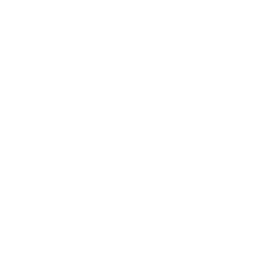
\includegraphics[scale=1]{assets/branding/opa0}
    \vspace{-5.75cm}\\
    {\adjustbox{scale=1.65}{\color{TealDarkCyan}\;II.\;When Decoding Is Easy}}
    \vspace{.25cm}
    \begin{minipage}{.78\textwidth}
      \scriptsize\color{Ink}
      \textbf{Big picture.}\;
      Algebraic structure turns the syndrome from a clue into an address: it names the error exactly.\\[.2cm]
      \textbf{Details to watch.}\;
      generator matrix, parity-check matrix, syndrome, Hamming bound, perfect code, cyclic ideal, quasi-cyclic hint.
    \end{minipage}
    {\ }\vspace{2.1cm}\\
    \bigskip
  \end{center}
\end{frame}

%=== A. LINEAR CODES ===

%--- Linear code definition ---
\begin{frame}{\textbf{II. When Decoding Is Easy}}{Linear Codes}
\small
\defbox[{Linear $[n,k,d]_q$ Code}]{
A \textbf{linear code} is a $k$-dimensional subspace $\code\le\F_q^n$ with minimum Hamming distance $d$.
Its elements are \textbf{codewords}.
}
\begin{columns}[T,onlytextwidth]
\begin{column}{.52\textwidth}
\defbox[Generator matrix]{
$\mat G\in\F_q^{k\times n}$: rows form a basis of $\code$.
Encoding: $\vect m \mapsto \vect c = \vect m\mat G$.
}
\defbox[Parity-check matrix]{
$\mat H\in\F_q^{(n-k)\times n}$: $\code = \ker(\mat H)$.
Check: $\vect c\in\code \Leftrightarrow \mat H\vect c^T = \vect 0$.
}
\end{column}
\begin{column}{.44\textwidth}
\textcolor{TealDarkCyan}{\textbf{Parameters}}
\begin{itemize}
  \item Rate $R=k/n$ (information density)
  \item Redundancy $r=n-k$ (check symbols)
  \item Distance $d$ (error budget)
\end{itemize}
\bigskip
\textcolor{TealDarkCyan}{\textbf{Error capability}}
\[
  t = \left\lfloor\frac{d-1}{2}\right\rfloor\;\text{errors corrected}
\]
\end{column}
\end{columns}
\end{frame}

%--- Systematic form + tikz ---
\begin{frame}{\textbf{II. When Decoding Is Easy}}{Systematic Form and Encoding}
\small
\defbox[Systematic form]{
$\mat G = [\mat I_k \mid \mat P]$: first $k$ coordinates carry the message; last $n-k$ are parity.
}
\begin{center}
\begin{tikzpicture}[x=1cm,y=1cm]
  \node[process] (msg) at (-4.55,0) {$\vect m$\\[-1pt]\scriptsize message};
  \foreach \i/\b in {1/1,2/0,3/1,4/1}{
    \node[bit teal,right={-0.01cm of msg},xshift={0.45*\i cm-0.2cm}]
      at (-5.8+0.05*\i,-1) {$\b$};
  }
  \node[process blue,minimum width=2.35cm,minimum height=1.48cm] (G) at (0,0)
    {\large $\mat G=[\mat I_k\mid \mat P]$};
  \node[process amber] (code) at (4.45,0) {$\vect c=\vect m\mat G$\\[-1pt]\scriptsize codeword};
  \foreach \i/\b in {1/1,2/0,3/1,4/1,5/0,6/0,7/1}{
    \ifnum\i<5
      \node[bit teal]  at (2.6+0.46*\i,-1) {$\b$};
    \else
      \node[bit amber] at (2.6+0.46*\i,-1) {$\b$};
    \fi
  }
  \draw[decorate,decoration={brace,amplitude=4pt},TealDarkCyan!75,line width=0.7pt]
    (4.66,-1.35) -- (2.86,-1.35) node[midway,below=0.12cm,tiny label]{message};
  \draw[decorate,decoration={brace,amplitude=4pt},AmberCode!85,line width=0.7pt]
    (6.06,-1.35) -- (4.66,-1.35) node[midway,below=0.12cm,tiny label]{parity};
  \draw[flow]      (msg) -- (G)    node[midway,above=0.12cm,tiny label]{linear map};
  \draw[flow blue] (G)   -- (code) node[midway,above=0.12cm,tiny label]{redundancy};
\end{tikzpicture}
\end{center}
\textbf{Example.}\; For the $[7,4,3]_2$ Hamming code with $\vect m=(1,0,1,1)$:
$\vect c = \vect m\mat G = (1,0,1,1,0,1,0)$.
\end{frame}

%--- Parity-check matrix + syndrome ---
\begin{frame}{\textbf{II. When Decoding Is Easy}}{Syndrome: The Error Fingerprint}
\small
\defbox[Syndrome]{
For received $\vect y = \vect c + \vect e$,
\[
  \vect s = \mat H\vect y^T = \underbrace{\mat H\vect c^T}_{=\,\vect 0} + \mat H\vect e^T = \mat H\vect e^T.
\]
The syndrome depends \emph{only on the error}, not on which codeword was sent.
}
\[
  \mat H = \begin{bmatrix}
    0&1&1&1&1&0&0\\
    1&0&1&1&0&1&0\\
    1&1&0&1&0&0&1
  \end{bmatrix}
  \xrightarrow{\;\mat H\vect e^T\;}
  \vect s = \begin{pmatrix}1\\0\\0\end{pmatrix}
\]
\begin{itemize}
  \item $\vect s = \vect 0$ iff $\vect y\in\code$ (no detectable error).
  \item Every nonzero $\vect s$ identifies the coset $\vect e + \code$.
  \item \textbf{Decoding} = find the minimum-weight $\vect e$ with $\mat H\vect e^T = \vect s$.
\end{itemize}
\end{frame}

%--- Distance theorem + packing ---
\begin{frame}{\textbf{II. When Decoding Is Easy}}{Error Correction and the Hamming Bound}
\small
\begin{columns}[T,onlytextwidth]
\begin{column}{.50\textwidth}
\thmbox[Distance theorem]{
A code of distance $d$ corrects every error of weight $\le t = \lfloor(d-1)/2\rfloor$
and detects every error of weight $\le d-1$.
}
\vspace{.4em}
\thmbox[Hamming bound]{
$\displaystyle q^k\sum_{i=0}^t\binom{n}{i}(q-1)^i \le q^n.$
}
\defbox[Perfect code]{
Equality in the Hamming bound: correction balls of radius $t$ tile $\F_q^n$ with \emph{no gaps and no overlap}.
}
\end{column}
\begin{column}{.46\textwidth}
\begin{center}
\begin{tikzpicture}[scale=.88]
  \fill[TealDarkCyan!6] (-2.8,-2.3) rectangle (2.8,2.3);
  \node[font=\tiny,TealDarkCyan!60] at (2.2,2.0) {$\F_2^n$};
  \fill[AccentCyan!25] (-1.4, 0.9) circle (.75);
  \fill[TealDarkCyan]  (-1.4, 0.9) circle (3pt) node[above=3pt,font=\tiny]{$c_1$};
  \fill[AccentCyan!25] ( 1.3, 0.9) circle (.75);
  \fill[TealDarkCyan]  ( 1.3, 0.9) circle (3pt) node[above=3pt,font=\tiny]{$c_2$};
  \fill[AccentCyan!25] ( 0.0,-1.1) circle (.75);
  \fill[TealDarkCyan]  ( 0.0,-1.1) circle (3pt) node[above=3pt,font=\tiny]{$c_3$};
  \node[font=\tiny,AccentCyan!70!TealDarkCyan] at (-2.3,-0.6) {balls};
  \node[font=\tiny,AccentCyan!70!TealDarkCyan] at (-2.3,-0.9) {radius $t$};
  \draw[dashed,TealDarkCyan!50] (-2.8,0)--(2.8,0);
  \node[font=\tiny,TealDarkCyan!50] at (2.1,-.2) {no overlap};
\end{tikzpicture}
\end{center}
\end{column}
\end{columns}
\end{frame}

%=== B. HAMMING CODES ===

%--- Historical motivation ---
\begin{frame}{\textbf{II. When Decoding Is Easy}}{Hamming (1950): The Original Insight}
\small
\begin{columns}[T,onlytextwidth]
\begin{column}{.54\textwidth}
Richard Hamming at Bell Labs in 1947: punched-card overnight jobs crashed on \emph{single-bit errors}.

\medskip
\textbf{His question:} ``If the machine can \emph{detect} an error, why can't it \emph{fix} it?''

\medskip
\defbox[Hamming's key idea]{
Add redundant parity bits so that:
\begin{itemize}
  \item the syndrome names the \textbf{exact error position}, and
  \item \textbf{no syndrome is wasted} — every nonzero syndrome maps to a unique error.
\end{itemize}
}
One error at position $i$, or no error: $n+1$ cases, $2^r$ syndromes.
\[
  n+1=2^r \;\Longrightarrow\; n=2^r-1.
\]
\end{column}
\begin{column}{.43\textwidth}
\begin{tikzpicture}[scale=.88]
  \node[font=\small\bfseries,TealDarkCyan] at (1.5,4.0) {Syndrome $\to$ action};
  \draw[TealDarkCyan,thick] (0,3.65)--(3.0,3.65);
  \node[draw=TealDarkCyan!40,rounded corners=3pt,fill=TealDarkCyan!8,
        minimum width=2.8cm,minimum height=0.38cm,font=\scriptsize]
    at (1.5,3.25) {$000$ $\to$ no error};
  \foreach \i/\bits in {1/001, 2/010, 3/011, 4/100, 5/101, 6/110, 7/111}{
    \pgfmathsetmacro{\yy}{3.25-\i*0.42}
    \node[draw=AccentCyan!60,rounded corners=3pt,fill=AccentCyan!10,
          minimum width=2.8cm,minimum height=0.38cm,font=\scriptsize]
      at (1.5,\yy) {$\bits$ $\to$ flip bit $\i$};
  }
\end{tikzpicture}
\end{column}
\end{columns}
\end{frame}

%--- Hamming code definition ---
\begin{frame}{\textbf{II. When Decoding Is Easy}}{The Binary Hamming Code}
\small
\defbox[Binary Hamming matrix $\mat H_r$]{
$\mat H_r$ is the $r\times(2^r-1)$ matrix whose columns are \emph{all nonzero binary vectors} of length $r$.
}
\[
  \mat H_3=\begin{bmatrix}1&0&1&0&1&0&1\\0&1&1&0&0&1&1\\0&0&0&1&1&1&1\end{bmatrix}.
\]
\defbox[Binary Hamming code]{
$\operatorname{Ham}(r,2)=\ker(\mat H_r)$, with parameters $[2^r-1,\;2^r-1-r,\;3]_2$.
}
\begin{columns}[T,onlytextwidth]
\begin{column}{.50\textwidth}
\begin{itemize}
  \item Every nonzero syndrome identifies a unique column of $\mat H_r$.
  \item The column label is the binary address of the error.
  \item Corrects exactly one error; detects exactly two.
\end{itemize}
\end{column}
\begin{column}{.46\textwidth}
\thmbox[Perfect]{
$2^k(1+n) = 2^{2^r-1}$ — the correction balls tile all of $\F_2^n$.
}
\end{column}
\end{columns}
\end{frame}

%--- Perfect tiling ---
\begin{frame}{\textbf{II. When Decoding Is Easy}}{Perfect Tiling: Why Hamming Codes Are Special}
\small
\begin{columns}[T,onlytextwidth]
\begin{column}{.47\textwidth}
For $[3,1,3]_2$ in $\F_2^3$: two correction balls of radius 1
\textbf{tile the cube exactly} — no overlap, no gap.
\begin{center}
\begin{tikzpicture}[scale=.78]
  \draw[gray!35,thick] (0,0)--(2,0); \draw[gray!35,thick] (0,0)--(1,.9);
  \draw[gray!35,thick] (0,0)--(.5,1.6); \draw[gray!35,thick] (2,0)--(3,.9);
  \draw[gray!35,thick] (2,0)--(2.5,1.6); \draw[gray!35,thick] (1,.9)--(3,.9);
  \draw[gray!35,thick] (1,.9)--(1.5,2.5); \draw[gray!35,thick] (.5,1.6)--(2.5,1.6);
  \draw[gray!35,thick] (.5,1.6)--(1.5,2.5); \draw[gray!35,thick] (3,.9)--(3.5,2.5);
  \draw[gray!35,thick] (2.5,1.6)--(3.5,2.5); \draw[gray!35,thick] (1.5,2.5)--(3.5,2.5);
  \foreach \x/\y/\col in {0/0/TealDarkCyan, 2/0/TealDarkCyan,
                           1/.9/TealDarkCyan, .5/1.6/TealDarkCyan}{
    \node[circle,draw=\col,fill=\col!20,minimum size=.60cm,font=\tiny\bfseries]
      at (\x,\y) {};
  }
  \foreach \x/\y/\s in {0/0/$000$, 2/0/$100$, 1/.9/$010$, .5/1.6/$001$}{
    \node[font=\tiny] at (\x,\y) {\s};
  }
  \foreach \x/\y/\col in {3.5/2.5/AccentCyan, 1.5/2.5/AccentCyan,
                           2.5/1.6/AccentCyan, 3/.9/AccentCyan}{
    \node[circle,draw=\col,fill=\col!22,minimum size=.60cm,font=\tiny\bfseries]
      at (\x,\y) {};
  }
  \foreach \x/\y/\s in {3.5/2.5/$111$, 1.5/2.5/$011$, 2.5/1.6/$101$, 3/.9/$110$}{
    \node[font=\tiny] at (\x,\y) {\s};
  }
  \node[below=3pt,font=\tiny,TealDarkCyan] at (0,0) {\textbf{c=000}};
  \node[above=3pt,font=\tiny,AccentCyan]   at (3.5,2.5) {\textbf{c=111}};
\end{tikzpicture}
\end{center}
\end{column}
\begin{column}{.50\textwidth}
\textcolor{TealDarkCyan}{\textbf{Why ``perfect''?}}
\begin{itemize}
  \item Each ball: 1 codeword + 3 distance-1 neighbours = 4 words
  \item Two balls cover all $2^3=8$ points; $2\times4=8$ ✓
  \item For $\operatorname{Ham}(r,2)$: $2^{2^r-1-r}\times 2^r = 2^{2^r-1}$ ✓
\end{itemize}

\medskip
\defbox[The decoder is one table look-up]{
Syndrome $\vect s\ne\vect 0$: find the unique column $i$ of $\mat H_r$ equal to $\vect s$.
Flip bit $i$.  Time: $O(1)$.
}

\medskip
No other linear perfect single-error-correcting code exists (apart from trivial cases).
\end{column}
\end{columns}
\end{frame}

%--- Encoding + syndrome walkthrough ---
\begin{frame}{\textbf{II. When Decoding Is Easy}}{Encoding and Correction: The Full Picture}
\small
\begin{center}
\begin{tikzpicture}[
  box/.style={draw=TealDarkCyan,thick,rounded corners=4pt,
              minimum width=2.0cm,minimum height=0.65cm,
              fill=TealDarkCyan!10,font=\scriptsize,align=center},
  earr/.style={-Stealth,thick,AccentCyan,dashed}
]
  \node[box] (msg)  at (0,0)   {Message\\$m=(1,0,1,1)$};
  \node[box] (enc)  at (3,0)   {Encoder\\$c=mG$};
  \node[box] (cw)   at (6,0)   {Codeword\\$c=(1,0,1,1,0,1,0)$};
  \node[box,fill=AccentCyan!12,draw=AccentCyan] (ch) at (9,0)
    {Channel\\flip bit 5};
  \node[box,fill=AccentCyan!8,draw=AccentCyan]  (rv)  at (9,-1.5)
    {Received\\$v=(1,0,1,1,\mathbf{1},1,0)$};
  \node[box] (syn)  at (6,-1.5) {Syndrome\\$s=(1,0,1)^T$};
  \node[box] (lkp)  at (3,-1.5) {Look up\\col 5 of $H$};
  \node[box] (fix)  at (0,-1.5) {Correct\\$\hat c=c$ \checkmark};
  \draw[-Stealth,thick,TealDarkCyan] (msg)--(enc);
  \draw[-Stealth,thick,TealDarkCyan] (enc)--(cw);
  \draw[-Stealth,thick,TealDarkCyan] (cw)--(ch);
  \draw[earr] (ch)--(rv);
  \draw[-Stealth,thick,TealDarkCyan] (rv)--(syn);
  \draw[-Stealth,thick,TealDarkCyan] (syn)--(lkp);
  \draw[-Stealth,thick,TealDarkCyan] (lkp)--(fix);
  \node[above=2pt,font=\tiny,TealDarkCyan] at (1.5,0)  {$mG$};
  \node[above=2pt,font=\tiny,AccentCyan]   at (9,-.75) {noise};
  \node[above=2pt,font=\tiny,TealDarkCyan] at (7.5,-1.5){$Hv^T$};
\end{tikzpicture}
\end{center}
\begin{columns}[T,onlytextwidth]
\begin{column}{.50\textwidth}
\begin{itemize}
  \item Syndrome $(1,0,1)^T$ = column 5 of $\mat H_3$
  \item Flip bit 5 to recover $c$ ✓
  \item The decoder \emph{never} needs to know $m$
\end{itemize}
\end{column}
\begin{column}{.46\textwidth}
\textcolor{TealDarkCyan}{\textbf{This is why Hamming codes work:}}
the syndrome is literally the binary address of the error.
No search, no iteration.
\end{column}
\end{columns}
\end{frame}

%--- The Fano plane ---
\begin{frame}{\textbf{II. When Decoding Is Easy}}{Geometry Behind the Code: The Fano Plane}
\small
\begin{columns}[T,onlytextwidth]
\begin{column}{.44\textwidth}
\begin{center}
\begin{tikzpicture}[scale=.85]
  \draw[TealDarkCyan,thick] (0,2) -- (-1.73,-1);
  \draw[TealDarkCyan,thick] (0,2) -- (1.73,-1);
  \draw[TealDarkCyan,thick] (-1.73,-1) -- (1.73,-1);
  \draw[AccentCyan,thick]  (0,2) -- (0,-1);
  \draw[AccentCyan,thick]  (-1.73,-1) -- (.865,.5);
  \draw[AccentCyan,thick]  (-.865,.5) -- (1.73,-1);
  \draw[TealDarkCyan!55,thick] (0,0) circle (1.0);
  \fill[TealDarkCyan] (0,2)     circle (3.5pt);
  \node[above=3pt,font=\scriptsize,TealDarkCyan] at (0,2) {$1$};
  \fill[TealDarkCyan] (-1.73,-1)circle (3.5pt);
  \node[left=3pt,font=\scriptsize,TealDarkCyan]  at (-1.73,-1){$2$};
  \fill[TealDarkCyan] (1.73,-1) circle (3.5pt);
  \node[right=3pt,font=\scriptsize,TealDarkCyan] at (1.73,-1) {$4$};
  \fill[AccentCyan] (-.865,.5)  circle (3.5pt);
  \node[left=3pt,font=\scriptsize,AccentCyan]    at (-.865,.5){$3$};
  \fill[AccentCyan] (.865,.5)   circle (3.5pt);
  \node[right=3pt,font=\scriptsize,AccentCyan]   at (.865,.5) {$5$};
  \fill[AccentCyan] (0,-1)      circle (3.5pt);
  \node[below=3pt,font=\scriptsize,AccentCyan]   at (0,-1)    {$6$};
  \fill[TealDarkCyan!70] (0,0)  circle (3.5pt);
  \node[right=4pt,font=\scriptsize,TealDarkCyan] at (0,0)     {$7$};
\end{tikzpicture}
\end{center}
\end{column}
\begin{column}{.53\textwidth}
\textcolor{TealDarkCyan}{\textbf{The 7 lines $\leftrightarrow$ 7 weight-3 codewords:}}
\smallskip
\begin{tabular}{c|c}
  Line & Columns sum to $\vect 0$ \\\hline
  \rowcolor{TealDarkCyan!8} $\{1,2,3\}$ & $100\oplus010=110$ \\
  $\{1,4,5\}$ & $100\oplus001=101$ \\
  \rowcolor{TealDarkCyan!8} $\{2,4,6\}$ & $010\oplus001=011$ \\
  $\{1,6,7\}$ & $100\oplus011=111$ \\
  \rowcolor{TealDarkCyan!8} $\{2,5,7\}$ & $010\oplus101=111$ \\
  $\{3,4,7\}$ & $110\oplus001=111$ \\
  \rowcolor{TealDarkCyan!8} $\{3,5,6\}$ & $110\oplus101=011$ \\
\end{tabular}
\bigskip

$d=3$ because the smallest Fano line has 3 points.
Algebraic structure = geometric minimum.
\end{column}
\end{columns}
\end{frame}

%=== C. CYCLIC CODES AND QUASI-CYCLIC ===

%--- Cyclic shift = polynomial multiplication ---
\begin{frame}{\textbf{II. When Decoding Is Easy}}{Cyclic Codes: Shift Symmetry}
\small
\defbox[Cyclic code]{
$\code\le\F_q^n$ is cyclic if $(c_0,\ldots,c_{n-1})\in\code \Rightarrow (c_{n-1},c_0,\ldots,c_{n-2})\in\code$.
}
Under the identification $(c_0,\ldots,c_{n-1})\leftrightarrow c(X)=c_0+c_1X+\cdots+c_{n-1}X^{n-1}$
in $R_n=\F_q[X]/(X^n-1)$:
\begin{itemize}
  \item cyclic shift = multiply by $X$ in $R_n$
  \item a cyclic code = an \textbf{ideal} in $R_n$ = $\ideal{g(X)}$ for a unique monic divisor $g(X)\mid X^n-1$
\end{itemize}
\begin{columns}[T,onlytextwidth]
\begin{column}{.50\textwidth}
\defbox[BCH bound]{
Prescribe $\delta-1$ consecutive roots $\alpha^b,\ldots,\alpha^{b+\delta-2}$ of $g(X)$.
Then $d\ge\delta$.
}
\end{column}
\begin{column}{.46\textwidth}
\textcolor{TealDarkCyan}{\textbf{Hardware bonus}}

Division by $g(X)$ computes via a shift register with $n-k$ flip-flops.
Encoding and syndrome computation run at wire speed.
\end{column}
\end{columns}
\textbf{Example.}\; $X^7-1=(X+1)(X^3+X+1)(X^3+X^2+1)$ over $\F_2$.
Taking $g=X^3+X+1$ gives the cyclic $[7,4,3]_2$ Hamming code.
\end{frame}

%--- Decoding summary for algebraic codes ---
\begin{frame}{\textbf{II. When Decoding Is Easy}}{Why Algebraic Structure Makes Decoding Easy}
\small
\begin{center}
\renewcommand{\arraystretch}{1.28}
\begin{tabular}{p{.22\textwidth}p{.26\textwidth}p{.40\textwidth}}
\toprule
Code family & Structure & Decoding mechanism \\
\midrule
Hamming $[2^r-1,*,3]_2$ & Projective parity checks & Syndrome = binary address; $O(1)$ table look-up \\
Cyclic (BCH, RS) & Ideal in $\F_q[X]/(X^n-1)$ & Root syndromes + Berlekamp--Massey; $O(n^2)$ \\
Reed--Solomon & Evaluation code; MDS & Welch--Berlekamp; $O(n^2)$ \\
LDPC / Turbo & Sparse Tanner graph & Belief propagation; near-linear \\
\bottomrule
\end{tabular}
\end{center}
\bigskip
\textbf{The pattern.}\;
Every efficient decoder exploits a specific algebraic invariant.
Projective geometry gives Hamming its $O(1)$ decoder.
Polynomial roots give BCH and RS their syndromes.
\medskip
\begin{alertblock}{}
\centering
Remove the algebraic structure \textbf{$\rightarrow$} no formula \textbf{$\rightarrow$} exponential search.
\end{alertblock}
\end{frame}

%--- Quasi-cyclic hint and transition ---
\begin{frame}{\textbf{II. When Decoding Is Easy}}{Quasi-Cyclic Codes: A Bridge to Cryptography}
\small
\defbox[Quasi-cyclic code of index $\ell$]{
$\code\subseteq\F_q^n$ ($n=\ell m$) is \textbf{quasi-cyclic} if it is invariant under cyclic shift by $\ell$ positions.
Generator matrices are built from $\ell\times\ell$ \textbf{circulant blocks} — each block described by one polynomial in $R_m=\F_q[X]/(X^m-1)$.
}
\begin{columns}[T,onlytextwidth]
\begin{column}{.52\textwidth}
\textcolor{TealDarkCyan}{\textbf{Why QC codes matter in cryptography}}
\begin{itemize}
  \item Entire parity-check matrix compressed from $O(n^2)$ to $O(n)$ bits.
  \item Arithmetic in $R_m$: polynomial multiplication, inversion.
  \item Random-looking but algebraically structured.
  \item Retains hardness of decoding — but now opens new attack surfaces.
\end{itemize}
\end{column}
\begin{column}{.44\textwidth}
\begin{center}
\begin{tikzpicture}[node distance=.5cm,scale=.80,transform shape]
  \node[process]              (cyc)  {cyclic code\\ideal in $R_n$};
  \node[process blue,below=of cyc]  (qc)   {quasi-cyclic\\$\ell$ circulant blocks};
  \node[process amber,below=of qc]  (hard) {QCSD\\hard search problem};
  \node[process red,below=of hard]  (pqc)  {BIKE/HQC\\PQC system};
  \draw[flow]       (cyc) -- (qc);
  \draw[flow blue]  (qc)  -- (hard);
  \draw[flow amber] (hard)-- (pqc);
\end{tikzpicture}
\end{center}
\end{column}
\end{columns}
\medskip
\textbf{Coming up:} We now ask what happens when we \emph{remove} algebraic structure entirely and face a random parity-check matrix.
\end{frame}


%-------------------------------------------------------
% III. SYNDROME DECODING PROBLEM
%-------------------------------------------------------
\section{III. Syndrome Decoding Problem}
\HardProblemLens{Remove algebraic structure and the syndrome becomes a dead end: no formula, only exponential search.}
%=======================================================
% CHAPTER 2: WHEN DECODING IS HARD — THE SYNDROME DECODING PROBLEM
%=======================================================

\begin{frame}[plain]
  \begin{center}\bfseries\centering
    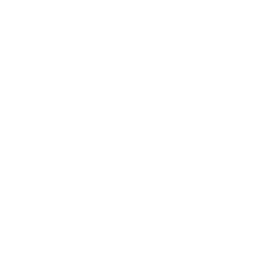
\includegraphics[scale=1]{assets/branding/opa0}
    \vspace{-5.75cm}\\
    {\adjustbox{scale=1.65}{\color{TealDarkCyan}\;III.\;Syndrome Decoding Problem}}
    \vspace{.25cm}
    \begin{minipage}{.78\textwidth}
      \scriptsize\color{Ink}
      \textbf{Big picture.}\;
      Remove the algebraic structure of Hamming and cyclic codes, and the same equation $\mat H\vect e^T=\vect s$ becomes NP-complete.\\[.2cm]
      \textbf{Details to watch.}\;
      random parity-check matrix, weight constraint, NP-completeness, ISD, McEliece, key size.
    \end{minipage}
    {\ }\vspace{2.1cm}\\
    \bigskip
  \end{center}
\end{frame}

%--- The turn: what changes? ---
\begin{frame}{\textbf{III. Syndrome Decoding Problem}}{The Turn: From Structure to Randomness}
\small
\begin{columns}[T,onlytextwidth]
\begin{column}{.50\textwidth}
\textcolor{TealDarkCyan}{\textbf{Structured $\mat H$ (Act II)}}
\begin{itemize}
  \item Columns are all nonzero binary vectors (Hamming).
  \item Generator polynomial of a cyclic ideal (BCH, RS).
  \item Syndrome points to the error address directly.
  \item Decoder runs in $O(1)$ or polynomial time.
\end{itemize}
\end{column}
\begin{column}{.46\textwidth}
\textcolor{TealDarkCyan}{\textbf{Random $\mat H$ (Act III)}}
\begin{itemize}
  \item Each entry of $\mat H$ is an independent uniform bit.
  \item No projective, polynomial, or cyclic structure.
  \item Syndrome gives no algebraic hint about $\vect e$.
  \item Best decoder takes exponential time.
\end{itemize}
\end{column}
\end{columns}
\bigskip
\begin{center}
\begin{tikzpicture}[node distance=.7cm]
  \node[process]          (str)   {structured\\$\mat H$};
  \node[process blue,   right=1.3cm of str]  (sd)    {syndrome\\decoding};
  \node[process amber,  above right=.35cm and 1.3cm of sd] (easy)
    {formula\\$O(1)$};
  \node[process red,    below right=.35cm and 1.3cm of sd] (hard)
    {no formula\\$2^{\Theta(n)}$};
  \node[process,        left=1.3cm of str]   (rand)  {random\\$\mat H$};
  \draw[flow]       (str)  -- (sd);
  \draw[flow]       (rand) -- (sd);
  \draw[flow amber] (sd.north east) -- (easy);
  \draw[flow red]   (sd.south east) -- (hard);
\end{tikzpicture}
\end{center}
\end{frame}

%--- SDP definition ---
\begin{frame}{\textbf{III. Syndrome Decoding Problem}}{The Syndrome Decoding Problem (SDP)}
\defbox[Syndrome Decoding Problem]{
\textbf{Input:}\; $\mat H\in\F_q^{r\times n}$,\; a syndrome $\vect s\in\F_q^r$,\; a weight bound $w\in\N$.\\[4pt]
\textbf{Search:}\; find $\vect e\in\F_q^n$ with
\[
  \mat H\vect e^T = \vect s \quad\text{and}\quad \wt(\vect e)\le w.
\]
\textbf{Decision:}\; does such $\vect e$ exist?
}
\begin{columns}[T,onlytextwidth]
\begin{column}{.50\textwidth}
\textcolor{TealDarkCyan}{\textbf{Parameters}}
\begin{itemize}
  \item $n$: code length
  \item $r=n-k$: redundancy (rows of $\mat H$)
  \item $w$: target error weight
  \item $q=2$: the binary case is most studied
\end{itemize}
\end{column}
\begin{column}{.46\textwidth}
\textcolor{TealDarkCyan}{\textbf{Why hard?}}
\begin{itemize}
  \item $\binom{n}{w}(q-1)^w$ candidates — exponential in $w$
  \item No algebraic shortcut for random $\mat H$
  \item For $n=1024$, $w=50$: $\binom{1024}{50}>10^{80}$
\end{itemize}
\end{column}
\end{columns}
\medskip
\textbf{Comparison.}\; For the $[7,4,3]_2$ Hamming code with $w=1$: only 7 candidates; syndrome names the answer in $O(1)$.
For a random $[1024,512]_2$ code with $w=50$: no formula, only search.
\end{frame}

%--- NP-completeness ---
\begin{frame}[shrink=5]{\textbf{III. Syndrome Decoding Problem}}{NP-Completeness of SDP}
\thmbox[Berlekamp--McEliece--van Tilborg (1978)]{
The decision version of the Syndrome Decoding Problem over $\F_2$ is NP-complete.
}
\begin{columns}[T,onlytextwidth]
\begin{column}{.54\textwidth}
\textbf{Proof sketch (reduction from 3-Dimensional Matching).}
\begin{itemize}
  \item Encode a 3-DM instance as a binary matrix $\mat H$ and syndrome $\vect s$.
  \item A perfect 3-D matching corresponds to a weight-$w$ error with $\mat H\vect e^T=\vect s$.
  \item The reduction is polynomial time.
\end{itemize}
\textbf{Consequence.}\; No polynomial-time algorithm for SDP exists unless $\mathrm{P}=\mathrm{NP}$.

\medskip
\textbf{\color{red}Caution.}\; NP-completeness is a \emph{worst-case} statement.
Cryptographic security requires hardness on \emph{average} for random instances — a separate (conjectured) claim.
\end{column}
\begin{column}{.42\textwidth}
\begin{center}
\begin{tikzpicture}[scale=.80,transform shape,node distance=.60cm]
  \node[process red,minimum width=2.6cm,align=center]     (sat) {3-DM\\(NP-complete)};
  \node[process blue,below=of sat,minimum width=2.6cm,align=center]  (poly){poly-time\\reduction};
  \node[process amber,below=of poly,minimum width=2.6cm,align=center] (sdp) {SDP over $\F_2$\\(NP-complete)};
  \draw[flow red]  (sat) -- (poly);
  \draw[flow blue] (poly) -- (sdp);
  \draw[flow amber,bend left=40]
    (sdp.east) to node[right,tiny label,align=center]{solve\\$\Rightarrow$\\P=NP} (sat.east);
\end{tikzpicture}
\end{center}
\end{column}
\end{columns}
\end{frame}

%--- Visualization: exponential search space ---
\begin{frame}{\textbf{III. Syndrome Decoding Problem}}{The Combinatorial Explosion}
\small
\begin{columns}[T,onlytextwidth]
\begin{column}{.44\textwidth}
For rate $R=1/2$ and error weight $w\approx 0.11n$ (near the Gilbert--Varshamov distance),
the search space is
\[
  \binom{n}{w}\approx 2^{H(w/n)\cdot n}
\]
where $H$ is the binary entropy function.
\medskip

At $n=1000$, $w=110$: $\binom{1000}{110}\approx 10^{100}$ candidates.
\medskip

\textbf{Compare with Hamming.}\; At $n=7$, $w=1$: exactly 7 candidates, resolved by the syndrome in $O(1)$.
\end{column}
\begin{column}{.52\textwidth}
\begin{center}
\begin{tikzpicture}[scale=.70]
  \draw[->,Ink!65] (-.3,0) -- (4.8,0) node[right,tiny label]{$n$};
  \draw[->,Ink!65] (0,-.3) -- (0,3.5) node[above,tiny label]{$\log_2\binom{n}{w}$};
  \draw[TealDarkCyan,thick,domain=.3:4.5,samples=30]
    plot (\x,{0.78*\x}) node[above right,tiny label,TealDarkCyan]{$nH(w/n)$};
  \fill[GoodGreen]  (.10,.08) circle (2.5pt);
  \node[above right,tiny label,GoodGreen]  at (.1,.08) {$n=7$ Hamming};
  \fill[ErrorRed]  (3.5,2.73) circle (2.5pt);
  \node[above right,tiny label,ErrorRed!80]at (3.5,2.73) {$n=1000$};
  \draw[ErrorRed!55,dashed] (0,1.5)--(4.8,1.5)
    node[right,tiny label,ErrorRed!70]{feasible};
  \node[caption text,align=center] at (2.4,-.75)
    {search space grows exponentially in $n$};
\end{tikzpicture}
\end{center}
\end{column}
\end{columns}
\end{frame}

%--- ISD ---
\begin{frame}[shrink=5]{\textbf{III. Syndrome Decoding Problem}}{Information-Set Decoding (ISD)}
\defbox[Prange's Algorithm (1962)]{
Randomly pick $k$ columns $I\subseteq[n]$ so that $\mat H_I$ is invertible (an \emph{information set}).
Assume $\vect e$ is zero on $I$, solve for $\vect e_{[n]\setminus I}=\mat H_{[n]\setminus I}^{-1}\vect s$.
If $\wt(\vect e)\le w$, output $\vect e$.  Otherwise retry.
}
\begin{columns}[T,onlytextwidth]
\begin{column}{.52\textwidth}
\textcolor{TealDarkCyan}{\textbf{Complexity}}
\begin{itemize}
  \item Success probability: $p=\binom{n-w}{k}/\binom{n}{k}$
  \item Cost per trial: $O(n^2)$ (Gaussian elimination)
  \item Total: $\approx O(n^2/p) = 2^{\Theta(n)}$
\end{itemize}
\medskip
\textcolor{TealDarkCyan}{\textbf{Best known ISD variants (binary, rate $1/2$)}}
\begin{itemize}
  \item Stern/Dumer (1989): $\approx 2^{0.054n}$ via birthday trick
  \item BJMM (2012): $\approx 2^{0.049n}$ via representations
  \item Quantum ISD: $\approx 2^{0.027n}$ (Grover, quadratic speedup only)
\end{itemize}
\end{column}
\begin{column}{.44\textwidth}
\begin{center}
\begin{tikzpicture}[node distance=.55cm,scale=.78,transform shape]
  \node[process]              (pick)  {pick info set $I$};
  \node[process blue,below=of pick]  (gauss) {Gauss on $\mat H_I$};
  \node[process amber,below=of gauss](solve) {solve for $\vect e_{[n]\setminus I}$};
  \node[process red,below=of solve]  (check) {$\wt(\vect e)\le w$?};
  \node[process,below=of check,fill=GoodGreen!10,draw=GoodGreen!70] (done) {output $\vect e$};
  \draw[flow]       (pick) -- (gauss);
  \draw[flow blue]  (gauss)-- (solve);
  \draw[flow amber] (solve)-- (check);
  \draw[flow,GoodGreen!80] (check)--node[right,tiny label]{yes}(done);
  \draw[flow red] (check.east)--++(0.5,0)
    |-node[near start,right,tiny label]{no: retry}(pick.east);
\end{tikzpicture}
\end{center}
\end{column}
\end{columns}
\end{frame}

%--- McEliece cryptosystem ---
\begin{frame}[shrink=5]{\textbf{III. Syndrome Decoding Problem}}{McEliece Cryptosystem (1978)}
\defbox[McEliece public-key encryption]{
\textbf{Key generation.}
Choose an $[n,k,d]$ code $\code$ with a $t$-error-correcting decoder (e.g., binary Goppa).
Let $\mat G\in\F_2^{k\times n}$ be its generator.  Choose random invertible $\mat S\in\F_2^{k\times k}$,
random permutation $\mat P\in\F_2^{n\times n}$.  Publish $\hat{\mat G}=\mat S\mat G\mat P$.

\textbf{Encryption.}
$\vect c=\vect m\hat{\mat G}+\vect e$,\; $\vect e$ random with $\wt(\vect e)=t$.

\textbf{Decryption.}
Apply $\mat P^{-1}$, decode $\code$, multiply by $\mat S^{-1}$.
}
\begin{columns}[T,onlytextwidth]
\begin{column}{.50\textwidth}
\textcolor{TealDarkCyan}{\textbf{Security}}
\begin{itemize}
  \item Breaking encryption = decoding $\hat{\mat G}$ without $(\mat S,\mat P)$ = SDP.
  \item Binary Goppa codes: efficient algebraic decoder, resistant to structural attacks.
  \item \textbf{Classic McEliece} is a NIST Round 4 finalist.
\end{itemize}
\end{column}
\begin{column}{.46\textwidth}
\textcolor{TealDarkCyan}{\textbf{Classic McEliece (128-bit)}}
\begin{center}
\renewcommand{\arraystretch}{1.1}
\begin{tabular}{ll}
  $n$ & 3488 \\
  $k$ & 2720 \\
  $t$ & 64 \\
  Public key & $\approx 261\,\text{KB}$ \\
  Ciphertext & $128\,\text{bytes}$ \\
\end{tabular}
\end{center}
\end{column}
\end{columns}
\end{frame}

%--- The cost: large keys ---
\begin{frame}{\textbf{III. Syndrome Decoding Problem}}{The Price of Generality: Large Keys}
\small
\begin{columns}[T,onlytextwidth]
\begin{column}{.52\textwidth}
\textcolor{TealDarkCyan}{\textbf{Why keys are large}}
\begin{itemize}
  \item Security requires $\hat{\mat G}$ to \emph{look random}.
  \item A random $k\times n$ binary matrix has $k(n-k)$ bits.
  \item For rate $R=1/2$: $k(n-k)\approx n^2/4$ bits $= O(n^2)$.
  \item At $n=3488$: $2720\times768 \approx 2.1\times10^6$ bits $\approx 261\,\text{KB}$.
\end{itemize}
\bigskip
\textcolor{TealDarkCyan}{\textbf{The tension}}
\begin{itemize}
  \item SDP hardness demands \emph{no structure}.
  \item No structure means \emph{no compression}.
  \item This is the fundamental trade-off of code-based cryptography.
\end{itemize}
\end{column}
\begin{column}{.44\textwidth}
\begin{center}
\begin{tikzpicture}[scale=.74]
  \draw[->,Ink!60] (0,0)--(0,3.6) node[above,tiny label]{key size};
  \fill[TealDarkCyan!70] (0.4,0) rectangle (1.4,2.8);
  \node[tiny label,align=center] at (.9,-.4) {Classic\\McEliece};
  \node[tiny label,white] at (.9,1.4) {261 KB};
  \fill[BlueCode!70] (2.0,0) rectangle (3.0,0.28);
  \node[tiny label,align=center] at (2.5,-.4) {BIKE};
  \node[tiny label,BlueCode] at (2.5,.52) {1.5 KB};
  \fill[AmberCode!70] (3.4,0) rectangle (4.4,0.52);
  \node[tiny label,align=center] at (3.9,-.4) {HQC};
  \node[tiny label,AmberCode] at (3.9,.76) {3.0 KB};
  \fill[GoodGreen!55] (4.8,0) rectangle (5.8,0.07);
  \node[tiny label,align=center] at (5.3,-.4) {Kyber\\(lattice)};
  \node[tiny label,GoodGreen!80] at (5.3,.3) {1.2 KB};
  \draw[<->,ErrorRed,line width=.8pt] (1.4,2.8)--(3.0,.28)
    node[midway,above right,tiny label,ErrorRed!85!black,rotate=-60]{$\times170$};
  \node[caption text,align=center,text width=4.6cm] at (3.0,-1.05)
    {compact keys require structure — but structure invites attacks};
\end{tikzpicture}
\end{center}
\end{column}
\end{columns}
\medskip
\textbf{The question for Act IV:} Can we add \emph{just enough} structure to compress the key while preserving hardness?
\end{frame}

%--- Complexity landscape ---
\begin{frame}[shrink=5]{\textbf{III. Syndrome Decoding Problem}}{SDP: Complexity Landscape}
\begin{center}
\renewcommand{\arraystretch}{1.24}
\begin{tabular}{p{.26\textwidth}p{.28\textwidth}p{.34\textwidth}}
\toprule
Problem variant & Complexity & Notes \\
\midrule
SDP decision & NP-complete & Berlekamp--McEliece--van Tilborg 1978 \\
SDP search, random $\mat H$, $w\approx\delta_\mathrm{GV}n$ & $2^{0.054n}$ (classical) & Best: Stern, BJMM, May--Ozerov \\
SDP search, quantum & $2^{0.027n}$ & Grover-accelerated ISD; no exponential improvement \\
Minimum distance (find min weight codeword) & NP-hard & Related: $\vect s=\vect 0$ version \\
Structured SDP (cyclic $\mat H$) & Unknown; may be easier & Algebraic attacks possible \\
QC-SDP (quasi-cyclic $\mat H$) & Believed $2^{\Theta(m)}$ & DOOM factor $\sqrt{m}$; Chapter IV \\
\bottomrule
\end{tabular}
\end{center}
\vspace{-.1cm}
\textbf{Summary.}\; SDP is the NP-complete engine at the heart of code-based cryptography.
Its worst-case hardness is proven; its average-case hardness is conjectured and empirically supported by 45 years of failed attacks.
The main weakness: it forces large keys.
Act IV resolves this with quasi-cyclic structure.
\end{frame}


%-------------------------------------------------------
% IV. QUASI-CYCLIC SYNDROME DECODING
%-------------------------------------------------------
\section{IV. Quasi-Cyclic Syndrome Decoding}
\HardProblemLens{Quasi-cyclic structure compresses keys from megabytes to kilobytes while keeping the essential hardness of SDP.}
%=======================================================
% CHAPTER 3: QUASI-CYCLIC SYNDROME DECODING — THE RESOLUTION
%=======================================================

\begin{frame}[plain]
  \begin{center}\bfseries\centering
    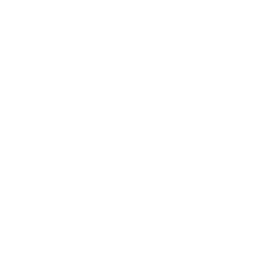
\includegraphics[scale=1]{assets/branding/opa0}
    \vspace{-5.75cm}\\
    {\adjustbox{scale=1.4}{\color{TealDarkCyan}\;IV.\;Quasi-Cyclic Syndrome Decoding}}
    \vspace{.25cm}
    \begin{minipage}{.78\textwidth}
      \scriptsize\color{Ink}
      \textbf{Big picture.}\;
      Quasi-cyclic structure compresses public keys from megabytes to kilobytes
      while keeping the essential hardness of SDP — but it opens new attack surfaces.\\[.2cm]
      \textbf{Details to watch.}\;
      circulant matrix, QCSD, key compression, BIKE, HQC, DOOM attack, hardness hierarchy.
    \end{minipage}
    {\ }\vspace{2.1cm}\\
    \bigskip
  \end{center}
\end{frame}

%--- The engineering resolution ---
\begin{frame}{\textbf{IV. Quasi-Cyclic Syndrome Decoding}}{The Engineering Resolution}
\small
\begin{columns}[T,onlytextwidth]
\begin{column}{.50\textwidth}
\textcolor{TealDarkCyan}{\textbf{Problem (Act III)}}
\begin{itemize}
  \item SDP is NP-complete and quantum-resistant.
  \item But random $\mat H$ forces $O(n^2)$-bit public keys.
  \item Classic McEliece: $261\,\text{KB}$ — impractical for many applications.
\end{itemize}
\end{column}
\begin{column}{.46\textwidth}
\textcolor{TealDarkCyan}{\textbf{Resolution (Act IV)}}
\begin{itemize}
  \item Add \emph{circulant} structure: each block described by one polynomial.
  \item Key size drops to $O(n)$ bits — a factor $\approx n/2$ reduction.
  \item Hardness \emph{inherited} from SDP; new attacks studied carefully.
\end{itemize}
\end{column}
\end{columns}
\bigskip
\begin{center}
\begin{tikzpicture}[node distance=.7cm]
  \node[process red,minimum width=3.0cm,align=center] (sdp)
    {SDP: NP-complete\\large keys $O(n^2)$};
  \node[process blue,right=1.2cm of sdp,minimum width=3.0cm,align=center] (qc)
    {QC structure\\circulant blocks};
  \node[process amber,right=1.2cm of qc,minimum width=3.0cm,align=center] (qcsd)
    {QCSD: hard\\compact keys $O(n)$};
  \node[process,right=1.2cm of qcsd,minimum width=2.6cm,align=center] (pqc)
    {BIKE / HQC\\NIST PQC};
  \draw[flow red]   (sdp) -- (qc);
  \draw[flow blue]  (qc)  -- (qcsd);
  \draw[flow amber] (qcsd)-- (pqc);
\end{tikzpicture}
\end{center}
\end{frame}

%--- Circulant matrices ---
\begin{frame}{\textbf{IV. Quasi-Cyclic Syndrome Decoding}}{Circulant Matrices: The Building Block}
\small
\defbox[Circulant matrix]{
$\mathrm{circ}(h_0,\ldots,h_{m-1})\in\F_q^{m\times m}$: each row is a cyclic shift of the row above.
\[
  \mat C = \begin{pmatrix}
    h_0 & h_1 & \cdots & h_{m-1} \\
    h_{m-1} & h_0 & \cdots & h_{m-2} \\
    \vdots & & \ddots & \vdots \\
    h_1 & h_2 & \cdots & h_0
  \end{pmatrix}
\]
}
\begin{columns}[T,onlytextwidth]
\begin{column}{.54\textwidth}
\begin{itemize}
  \item $\mat C$ corresponds to $h(X)=\sum h_i X^i\in R_m=\F_q[X]/(X^m-1)$.
  \item $\mathrm{circ}(h)\cdot\mathrm{circ}(g) = \mathrm{circ}(h\cdot g\bmod X^m-1)$.
  \item Entire $m\times m$ matrix compressed to $m$ bits.
  \item Arithmetic in $R_m$ is fast: NTT-based multiplication in $O(m\log m)$.
\end{itemize}
\end{column}
\begin{column}{.42\textwidth}
\begin{center}
\begin{tikzpicture}[scale=.72]
  % Left circulant H0
  \draw[TealDarkCyan,thick,fill=TealDarkCyan!8] (0,0) rectangle (2.6,2.2);
  \node[tiny label,TealDarkCyan] at (1.3,2.45) {$\mat H_0=\mathrm{circ}(h_0)$};
  \foreach \d in {0,...,3}{
    \pgfmathsetmacro{\y}{0.5+0.5*\d}
    \pgfmathsetmacro{\xs}{0.55*\d}
    \draw[TealDarkCyan!50,line width=1.4pt] (\xs,\y) -- (\xs+0.5,\y);
  }
  \node[tiny label,AccentCyan!80] at (1.3,1.1) {circulant};
  % Right circulant H1
  \draw[BlueCode,thick,fill=BlueCode!7] (2.9,0) rectangle (5.5,2.2);
  \node[tiny label,BlueCode] at (4.2,2.45) {$\mat H_1=\mathrm{circ}(h_1)$};
  \foreach \d in {0,...,3}{
    \pgfmathsetmacro{\y}{0.5+0.5*\d}
    \pgfmathsetmacro{\xs}{2.9+0.55*\d}
    \draw[BlueCode!50,line width=1.4pt] (\xs,\y) -- (\xs+0.5,\y);
  }
  \node[tiny label,BlueCode!80] at (4.2,1.1) {circulant};
  \draw[<->,Ink!55,line width=.6pt] (-0.3,0)--(-0.3,2.2)
    node[midway,left,tiny label]{$m$};
  \draw[<->,Ink!55,line width=.6pt] (0,-0.4)--(5.5,-0.4)
    node[midway,below,tiny label]{$n=2m$ (all described by 2 polynomials)};
\end{tikzpicture}
\end{center}
\end{column}
\end{columns}
\end{frame}

%--- QCSD definition ---
\begin{frame}[shrink=5]{\textbf{IV. Quasi-Cyclic Syndrome Decoding}}{The QCSD Problem}
\defbox[Quasi-Cyclic Syndrome Decoding (QCSD)]{
\textbf{Input:}\; block-circulant $\mat H=[\mat H_0\mid\cdots\mid\mat H_{\ell-1}]\in\F_q^{m\times\ell m}$,
$\mat H_i=\mathrm{circ}(h_i)$,\; syndrome $\vect s\in\F_q^m$,\; weight $w$.\\[4pt]
\textbf{Search:}\; find $\vect e=(\vect e_0|\cdots|\vect e_{\ell-1})\in\F_q^{\ell m}$ with
\[
  \sum_{i=0}^{\ell-1}\mat H_i\vect e_i^T = \vect s
  \quad\text{and}\quad \wt(\vect e)\le w.
\]
\textbf{Polynomial form:}\; find $e_i\in R_m$ with $\sum_i h_i e_i \equiv s\pmod{X^m-1}$ and $\sum_i\wt(e_i)\le w$.
}
\begin{columns}[T,onlytextwidth]
\begin{column}{.50\textwidth}
\textcolor{TealDarkCyan}{\textbf{Relation to SDP}}
\begin{itemize}
  \item QCSD is a structured instance of SDP.
  \item A QCSD solver implies an SDP solver (for this instance family).
  \item QC structure opens new algebraic and statistical attacks.
\end{itemize}
\end{column}
\begin{column}{.46\textwidth}
\textcolor{TealDarkCyan}{\textbf{Why it is still hard}}
\begin{itemize}
  \item No polynomial-time algorithm known.
  \item Algebraic attacks (Gröbner) fail at NIST parameters.
  \item NIST selected BIKE for standardization consideration.
\end{itemize}
\end{column}
\end{columns}
\end{frame}

%--- QC-MDPC codes ---
\begin{frame}{\textbf{IV. Quasi-Cyclic Syndrome Decoding}}{QC-MDPC Codes}
\small
\defbox[QC-MDPC Code (Misoczki et al., 2013)]{
A \textbf{Quasi-Cyclic Moderate Density Parity Check} code has parity-check matrix
$\mat H=[\mat H_0|\mat H_1]$ with $\mat H_i=\mathrm{circ}(h_i)$ and \emph{moderate} row weight $d_v\approx\sqrt{n}$.
}
\begin{columns}[T,onlytextwidth]
\begin{column}{.52\textwidth}
\textcolor{TealDarkCyan}{\textbf{Key features}}
\begin{itemize}
  \item Derived from LDPC philosophy but with higher weight than classical LDPC.
  \item Efficient probabilistic decoder: \textbf{iterative bit-flipping}.
  \item Security based on QCSD hardness, not on LDPC structure.
\end{itemize}
\textbf{Bit-flipping decoder.}\;
For each bit, count the parity checks it violates. Flip bits with the highest count. Iterate.
This is efficient but probabilistic — decoding failure rate $\delta_\mathrm{DFR}>0$.
\end{column}
\begin{column}{.44\textwidth}
\begin{center}
\begin{tikzpicture}[scale=.72]
  \draw[TealDarkCyan!40,fill=TealDarkCyan!5] (0,0) rectangle (2.2,1.8);
  \draw[BlueCode!40,fill=BlueCode!5]    (2.4,0) rectangle (4.6,1.8);
  \node[tiny label,TealDarkCyan] at (1.1,2.0) {$\mat H_0$};
  \node[tiny label,BlueCode] at (3.5,2.0) {$\mat H_1$};
  \foreach \x/\y in {.3/.4,.9/1.5,1.5/.8,.6/1.1,1.8/.3,
                     2.7/1.4,3.2/.5,3.8/1.0,4.3/1.6,2.9/.2}{
    \fill[TealDarkCyan!70] (\x,\y) circle (2pt);
  }
  \node[caption text,align=center,text width=4.5cm] at (2.3,-.55)
    {moderate weight: $d_v\approx\sqrt{n}$ ones per row};
\end{tikzpicture}
\end{center}
\end{column}
\end{columns}
\end{frame}

%--- BIKE ---
\begin{frame}[shrink=5]{\textbf{IV. Quasi-Cyclic Syndrome Decoding}}{BIKE: Bit Flipping Key Encapsulation}
\defbox[BIKE KEM (NIST PQC Round 4 finalist)]{
\textbf{Setup.}\; QC-MDPC code in $R_m^2$, $m$ prime, sparse $h_0,h_1\in R_m$ with $\wt=d_v$.

\textbf{Key generation.}\; Secret: $(h_0,h_1)$.  Public: $g=h_0^{-1}h_1\in R_m$.

\textbf{Encapsulation.}\;
Sample sparse $e_0,e_1\in R_m$ with $\wt(e_0)+\wt(e_1)=t$.
Ciphertext: $c=e_0+e_1\cdot g\in R_m$.

\textbf{Decapsulation.}\;
$c\cdot h_0 = e_0 h_0+e_1 h_1 = s$ (syndrome).
Run BGF bit-flipping decoder on $(s,h_0,h_1)$ to recover $(e_0,e_1)$.
}
\begin{columns}[T,onlytextwidth]
\begin{column}{.50\textwidth}
\textcolor{TealDarkCyan}{\textbf{Security}}
\begin{itemize}
  \item Breaking = solve QCSD on $(h_0,h_1)$, or find $(h_0,h_1)$ from $g$.
  \item Finding $(h_0,h_1)$ from $g=h_0^{-1}h_1$: \emph{polynomial factorization with weight constraints} in $R_m$ — no polynomial-time algorithm known.
\end{itemize}
\end{column}
\begin{column}{.46\textwidth}
\textcolor{TealDarkCyan}{\textbf{BIKE Level 1 parameters (128-bit)}}
\begin{center}
\renewcommand{\arraystretch}{1.1}
\begin{tabular}{ll}
  $m$ & 12323 \\
  $n=2m$ & 24646 \\
  $d_v$ & 71 \\
  $t$ & 134 \\
  Public key & 1541 bytes \\
  Ciphertext & 1573 bytes \\
\end{tabular}
\end{center}
\end{column}
\end{columns}
\end{frame}

%--- Decoding failure ---
\begin{frame}{\textbf{IV. Quasi-Cyclic Syndrome Decoding}}{Decoding Failure: A Critical Subtlety}
\small
\defbox[Decoding failure rate (DFR)]{
The BGF bit-flipping decoder fails with probability $\delta_\mathrm{DFR}$.
For BIKE Level 1: $\delta_\mathrm{DFR}\approx 2^{-128}$.
A non-zero DFR enables \emph{reaction attacks}.
}
\begin{columns}[T,onlytextwidth]
\begin{column}{.52\textwidth}
\textcolor{TealDarkCyan}{\textbf{The black-peg attack}}
\begin{itemize}
  \item Attacker submits chosen ciphertexts and observes decapsulation failures.
  \item Each failure leaks information about the secret key $(h_0,h_1)$.
  \item After polynomially many queries, the key can be recovered.
\end{itemize}
\textbf{Mitigation.}\;
BIKE uses a \emph{deterministic} BGF decoder variant.
The same ciphertext always decapsulates the same way, removing the oracle.
\end{column}
\begin{column}{.44\textwidth}
\begin{center}
\begin{tikzpicture}[scale=.74,transform shape,node distance=.52cm]
  \node[process]              (enc) {encapsulate\\$(e_0,e_1)$};
  \node[process blue,below=of enc]  (synd) {syndrome\\$s\in R_m$};
  \node[process amber,below=of synd](bgf) {BGF bit-flip\\decoder};
  \node[process red,below=of bgf]   (check){$(e_0',e_1')=?$};
  \node[process,below=of check,fill=GoodGreen!10,draw=GoodGreen!70] (ok) {accept};
  \node[process red,right=.8cm of check,minimum width=1.4cm,align=center]
    (fail){DFR\\$2^{-128}$};
  \draw[flow]       (enc)  -- (synd);
  \draw[flow blue]  (synd) -- (bgf);
  \draw[flow amber] (bgf)  -- (check);
  \draw[flow,GoodGreen!80] (check)--node[right,tiny label]{yes}(ok);
  \draw[flow red]   (check.east)--node[above,tiny label]{no}(fail);
\end{tikzpicture}
\end{center}
\end{column}
\end{columns}
\end{frame}

%--- HQC ---
\begin{frame}{\textbf{IV. Quasi-Cyclic Syndrome Decoding}}{HQC: Hamming Quasi-Cyclic}
\small
\defbox[HQC KEM (NIST PQC Round 4 alternate)]{
\textbf{Setup.}\; Work in $R_n=\F_2[X]/(X^n-1)$, $n$ prime.  Choose random $h\in R_n$.

\textbf{Key generation.}\;
Secret: sparse $x,y\in R_n$.\;
Public: $s=x+yh\in R_n$.

\textbf{Encapsulation.}\;
Sample sparse $r_1,r_2,e\in R_n$.
Ciphertext: $(\vect u,\vect v)=(r_1+r_2 h,\;mr_2+sr_1+e)$.

\textbf{Decapsulation.}\;
$\vect u\cdot y \approx \vect v\cdot r_2/r_2$ (inner product extraction), then decode the inner BCH or RS code.
}
\begin{columns}[T,onlytextwidth]
\begin{column}{.50\textwidth}
\textcolor{TealDarkCyan}{\textbf{HQC Level 1 (128-bit)}}
\begin{center}
\renewcommand{\arraystretch}{1.1}
\begin{tabular}{ll}
  $n$ & 17669 \\
  Weight of $x,y$ & 66 \\
  Weight of $r_1,r_2,e$ & 75 \\
  Public key & 2249 bytes \\
  Ciphertext & 4481 bytes \\
\end{tabular}
\end{center}
\end{column}
\begin{column}{.46\textwidth}
\textcolor{TealDarkCyan}{\textbf{Security}}
\begin{itemize}
  \item Hardness of QCSD: recover sparse $x,y$ from random-looking $s=x+yh$.
  \item Uses an inner RS or BCH code for \emph{deterministic} decryption.
  \item No DFR issue (deterministic inner decoder).
\end{itemize}
\end{column}
\end{columns}
\end{frame}

%--- Attacks on QCSD ---
\begin{frame}[shrink=5]{\textbf{IV. Quasi-Cyclic Syndrome Decoding}}{Attack Landscape for QCSD}
\begin{center}
\renewcommand{\arraystretch}{1.24}
\begin{tabular}{p{.22\textwidth}p{.18\textwidth}p{.48\textwidth}}
\toprule
Attack & Exploits & Notes \\
\midrule
ISD (Stern/BJMM) & No QC structure & Best generic attack; cost $\approx 2^{0.054n}$ \\
DOOM (Sendrier 2011) & QC orbit size $m$ & $m$ cyclically related instances; reduces ISD by $\sqrt{m}$ \\
Algebraic (Gröbner) & Ring $R_m$ & Effective only for tiny parameters; fails at NIST levels \\
Distinguisher & Statistical QC bias & Can detect QC structure; no decoding from this alone \\
Reaction attack & DFR $>0$ & Black-peg attack; mitigated by deterministic BGF decoder \\
Polynomial factoring & $g=h_0^{-1}h_1$ & Recover secret key; no poly-time algorithm known \\
Quantum ISD & Grover speedup & $\approx 2^{0.027n}$; parameters doubled to compensate \\
\bottomrule
\end{tabular}
\end{center}
\vspace{-.1cm}
\textbf{Lesson.}\; QC structure opens \emph{more} attack surfaces than random SDP.
Every known attack is accounted for in BIKE and HQC parameter choices.
\end{frame}

%--- DOOM visualization ---
\begin{frame}{\textbf{IV. Quasi-Cyclic Syndrome Decoding}}{The DOOM Attack: Cyclic Orbit as Free Speedup}
\small
\defbox[DOOM (Sendrier 2011)]{
Given $N$ SDP instances with the same $\mat H$ and different syndromes $\vect s_1,\ldots,\vect s_N$,
find \emph{any one} solution.  ISD cost: $\approx 2^{0.054n}/\sqrt{N}$.
}
\begin{columns}[T,onlytextwidth]
\begin{column}{.52\textwidth}
\textbf{Connection to QCSD.}\;
The cyclic orbit of any solution $\vect e$ gives $m$ solutions,
each with a cyclically shifted syndrome.
So QCSD implicitly provides $m$ related instances.

\medskip
\textbf{Impact.}\;
Effective ISD cost for QCSD: $\approx 2^{0.054n}/\sqrt{m}$.
Parameters must be enlarged to absorb this factor $\sqrt{m}$.

\medskip
\textbf{Magnitude.}\;
For BIKE ($m=12323$): DOOM gives a speedup of $\sqrt{12323}\approx 2^{6.9}$.
Parameters are chosen so that even after this correction, the cost exceeds $2^{128}$.
\end{column}
\begin{column}{.44\textwidth}
\begin{center}
\begin{tikzpicture}[scale=.72]
  % N instances on left
  \foreach \i in {1,2,3}{
    \pgfmathsetmacro{\yy}{2.2-0.75*(\i-1)}
    \node[process blue,minimum width=2.0cm,minimum height=0.44cm,
          align=center,font=\scriptsize] (s\i) at (0,\yy)
      {$\mat H\vect e^T=\vect s_{\i}$};
  }
  \node[tiny label] at (0,.05) {$\vdots$};
  \node[tiny label] at (0,-.4) {$m$ instances (orbit)};
  \node[process amber,minimum width=2.0cm,align=center] (doom) at (3.0,.9)
    {DOOM\\$\sqrt{m}$ speedup};
  \draw[flow blue]  (s1.east)  -- (doom.north west);
  \draw[flow blue]  (s2.east)  -- (doom.west);
  \draw[flow blue]  (s3.east)  -- (doom.south west);
  \node[process red,minimum width=2.0cm,align=center] (sol) at (3.0,-.25)
    {any solution\\$\vect e$};
  \draw[flow amber] (doom) -- (sol);
\end{tikzpicture}
\end{center}
\end{column}
\end{columns}
\end{frame}

%--- Hardness hierarchy ---
\begin{frame}{\textbf{IV. Quasi-Cyclic Syndrome Decoding}}{Code-Based Hardness Hierarchy}
\small
\begin{center}
\begin{tikzpicture}[node distance=.65cm]
  \node[process red,minimum width=3.2cm,align=center]
    (np)  {NP-complete\\(3-DM, SAT, $\ldots$)};
  \node[process amber,below=of np,minimum width=3.2cm,align=center]
    (sdp) {SDP\\generic random code};
  \node[process blue,below=of sdp,minimum width=3.2cm,align=center]
    (qcsd){QCSD\\QC code, circulant $\mat H$};
  \node[process,below left=0.65cm and -0.7cm of qcsd,minimum width=2.5cm,align=center]
    (bike){BIKE\\QC-MDPC};
  \node[process,below right=0.65cm and -0.7cm of qcsd,minimum width=2.5cm,align=center]
    (hqc) {HQC\\QC ring};
  \draw[flow red]   (np) -- node[right,tiny label]{NP-reduction} (sdp);
  \draw[flow amber] (sdp)-- node[right,tiny label]{instantiation} (qcsd);
  \draw[flow blue]  (qcsd.south west) -- (bike.north);
  \draw[flow blue]  (qcsd.south east) -- (hqc.north);
\end{tikzpicture}
\end{center}
\medskip
\textbf{Reading the hierarchy.}\;
Every downward arrow is a reduction:
breaking BIKE/HQC implies solving QCSD;
solving QCSD implies solving SDP (for this family);
solving general SDP implies P $=$ NP.
\end{frame}

%--- SDP vs QCSD comparison ---
\begin{frame}[shrink=5]{\textbf{IV. Quasi-Cyclic Syndrome Decoding}}{SDP vs.\ QCSD: The Complete Comparison}
\begin{center}
\renewcommand{\arraystretch}{1.28}
\begin{tabular}{p{.22\textwidth}p{.34\textwidth}p{.32\textwidth}}
\toprule
Property & SDP (generic) & QCSD \\
\midrule
Hardness basis & NP-complete (worst case) & Reduction to SDP; believed hard on average \\
Public key size & $O(n^2)$ bits & $O(n/\ell)$ bits (circulant compression) \\
Attack surface & ISD only & ISD + DOOM + algebraic + reaction \\
Best classical attack & Stern/BJMM $\approx 2^{0.054n}$ & ISD with DOOM factor $1/\sqrt{m}$ \\
Best quantum attack & $\approx 2^{0.027n}$ & Same + DOOM \\
Main PQC systems & Classic McEliece (Round 4) & BIKE (Round 4 finalist), HQC (alternate) \\
Key sizes at 128-bit & $\approx 261\,\text{KB}$ & $1.5$--$3\,\text{KB}$ \\
\bottomrule
\end{tabular}
\end{center}
\vspace{-.1cm}
\textbf{The trade-off.}\; QC structure buys a factor $\approx 170\times$ in key size
at the cost of a broader attack surface and more careful parameter design.
\end{frame}

%--- Final perspective: resolution ---
\begin{frame}{\textbf{IV. Quasi-Cyclic Syndrome Decoding}}{Resolution: The Four-Act Story Completed}
\small
\begin{columns}[T,onlytextwidth]
\begin{column}{.50\textwidth}
\defbox[Act I (Introduction)]{
The syndrome equation $\mat H\vect e^T=\vect s$
serves both reliable communication and cryptography.
The same math, two opposite goals.
}
\defbox[Act II (Development)]{
Algebraic structure — projective geometry (Hamming),
polynomial ideals (cyclic codes) — makes syndrome decoding $O(1)$ or polynomial.
}
\end{column}
\begin{column}{.46\textwidth}
\defbox[Act III (Turn)]{
Remove structure and decoding becomes NP-complete (SDP).
Hardness is proven. But random codes force $O(n^2)$-bit keys.
}
\defbox[Act IV (Conclusion)]{
Quasi-cyclic structure is the resolution:
circulant blocks compress keys to $O(n)$,
inherited SDP hardness survives,
and careful parameters defeat all known attacks.
}
\end{column}
\end{columns}
\bigskip
\begin{center}
\textbf{\large Code-based hardness is the art of hiding a sparse polynomial inside a circulant ring.}
\end{center}
\end{frame}


%-------------------------------------------------------
% CLOSING FRAME
%-------------------------------------------------------
\HardProblemLens{Algebraic structure gives efficiency; lack of it gives hardness; quasi-cyclic structure gives both.}
\begin{frame}[plain]
  \begin{center}\bfseries\centering
    \vspace{1.35cm}
    {\Huge\color{TealDarkCyan} Thank You}\\[.5cm]
    {\large\color{black} Ji, Yong-hyeon}\\[.3cm]
    {\normalsize\texttt{hacker3740@gmail.com}}\\[.5cm]
    \begin{minipage}{.80\textwidth}
      \small\color{Ink}
      \textbf{Big picture.}\;
      Hamming and cyclic codes show that algebraic structure turns syndrome decoding into a closed-form map.
      Remove that structure and the same syndrome equation becomes NP-hard.\\[.2cm]
      \textbf{Details to remember.}\;
      SDP is NP-complete (Berlekamp--McEliece--van Tilborg 1978);
      QCSD adds quasi-cyclic structure for compact keys;
      BIKE and HQC are the PQC instances.
    \end{minipage}\\[.5cm]
    {\small\color{gray} Enjoying Math $\cdot$ Hard Problems $\cdot$ 2026}
    \bigskip
  \end{center}
\end{frame}

\end{document}
